\chapter{Técnicas de visión computerizada}
Aquí se detallan todas las técnicas aplicadas o descartadas a lo largo
de la investigación. Incluye ejemplos de las tomografías para poder
relacionar la técnica con el resultado visual.\\
Toda la información presente en este capítulo ha sido redactada acorde
a las siguientes fuentes:
\begin{description}
\item[Hypermedia image processing
  reference]~\emph{\citep*{fisher1996hypermedia}}
\item[Computer Vision: Algorithms and
  Applications]~\emph{\citep*{szeliski2010computer}}
\item[Learning OpenCV]~\emph{\citep*{opencv_book-bib}}
\item[Tutorial de OpenCV para
  Python]~\emph{\citep*{opencv_tutorial-bib}}
\item[API de OpenCV]~\emph{\citep*{opencv_api-bib}}
\end{description}

\section{Conocimientos previos necesarios}

\subsection{Histogramas}\label{tecnica:histogramas}
Un histograma~\emph{\citep*[Chapter 7. Histograms and
  Matching]{opencv_book-bib}} es un gráfico con la distribución de
color o intensidades de la imagen. Por simplificación, supondremos
siempre una imagen en escala de grises. Es tan importante su estudio
dentro de la visión computerizada que se podría definir informalmente
como el gráfico que contiene la naturaleza de la imagen.
\begin{description}
\item[Columnas:] representan intensidades. Cada columna tiene una
  altura que corresponde proporcionalmente a la cantidad de píxeles
  con dicho valor.
\item[Dimensiones:] parámetros o número de datos a mostrar en el
  histograma. En el caso de una escala de grises sólo hay una
  dimensión, la intensidad, que puede ser 1 si el píxel tiene dicha
  intensidad o 0 en caso contrario.
\item[Rango:] es el número de columnas. En escala de grises el rango
  es de 256 columnas desde 0 hasta 255.
\end{description}

\subsubsection{Cálculo}
Para realizar el cálculo de un histograma y por simplificación se usa
una biblioteca. Tanto \emph{Numpy} como \emph{OpenCV} son capaces de
realizar los cálculos necesarios pero por eficiencia se usa
\emph{OpenCV}.

\subsubsection{Dibujado}
El resultado de un histograma es una matriz de \emph{Numpy} por lo
que, para poder dibujarla, tiene que usarse \emph{Matplotlib} o
transformar la matriz en una imagen de \emph{OpenCV}.

\begin{figure}[H]
  \caption{Original}
  \centering \setlength\fboxsep{0pt} \setlength\fboxrule{0.5pt}
  \fbox{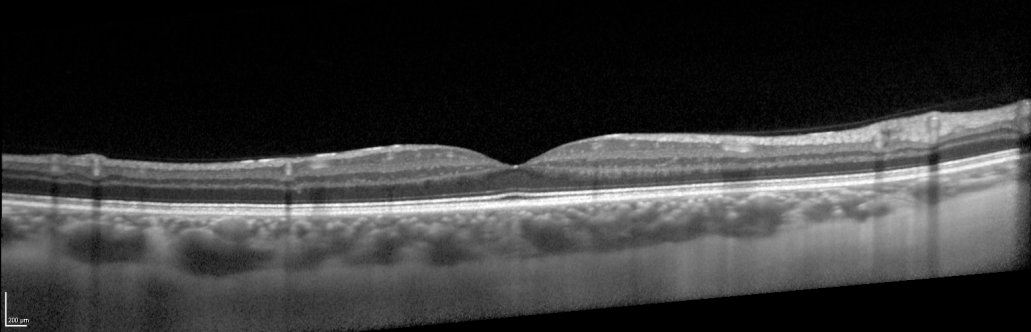
\includegraphics[width=\textwidth]{imagenes/tecnicas/histogramas/original_histogram.png}}
\end{figure}

\begin{figure}[H]
  \caption{Histograma}
  \centering \setlength\fboxsep{0pt} \setlength\fboxrule{0.5pt}
  \fbox{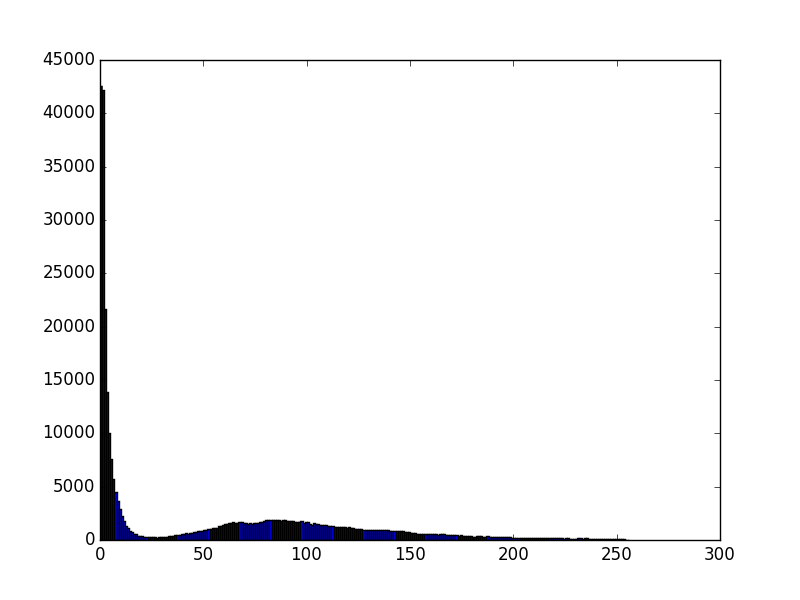
\includegraphics[scale=0.4]{imagenes/tecnicas/histogramas/histogram.png}}
\end{figure}

\subsubsection{Ecualización}
La ecualización~\emph{\citep*[3.1.4 Histogram
  equalization]{szeliski2010computer}} de un histograma consiste en
distribuir los píxeles por todo el rango. Esta acción aumenta el
contraste en aquellas imágenes que tienen la mayoría confinados en una
zona pequeña del rango.

\begin{figure}[H]
  \caption{Original}
  \centering \setlength\fboxsep{0pt} \setlength\fboxrule{0.5pt}
  \fbox{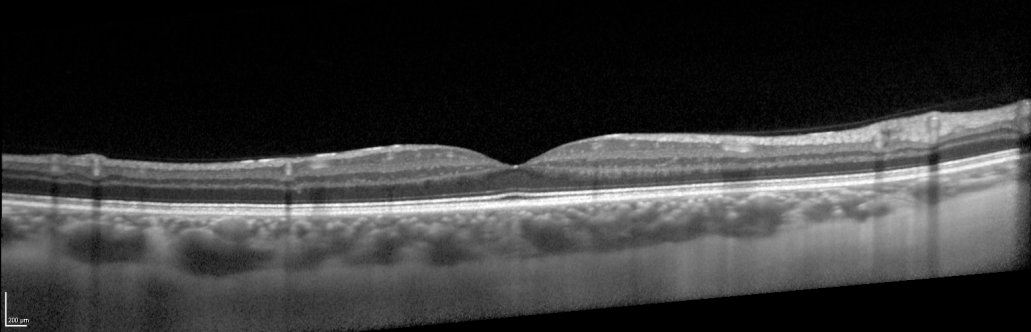
\includegraphics[width=\textwidth]{imagenes/tecnicas/histogramas/original_histogram.png}}
\end{figure}

\begin{figure}[H]
  \caption{Histograma ecualizado}
  \centering \setlength\fboxsep{0pt} \setlength\fboxrule{0.5pt}
  \fbox{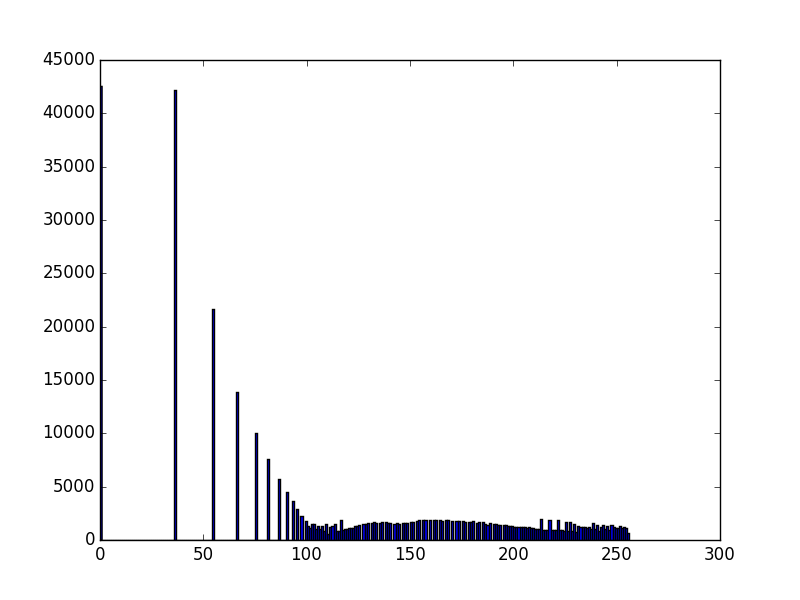
\includegraphics[scale=0.4]{imagenes/tecnicas/histogramas/equalization.png}}
\end{figure}

\begin{figure}[H]
  \caption{Original ecualizada}
  \centering \setlength\fboxsep{0pt} \setlength\fboxrule{0.5pt}
  \fbox{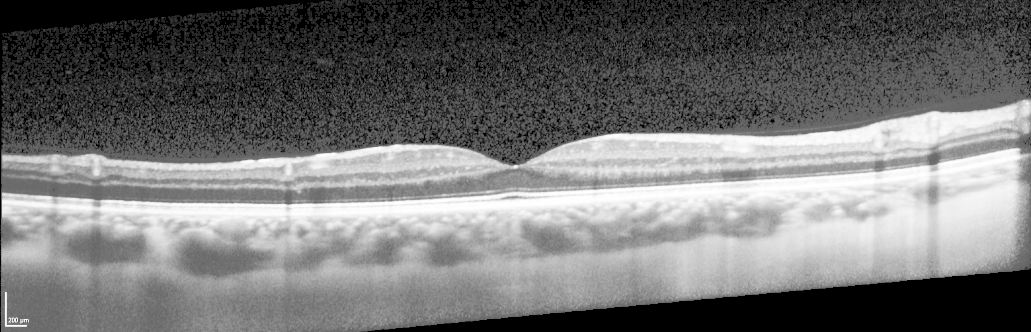
\includegraphics[width=\textwidth]{imagenes/tecnicas/histogramas/equalization_histogram.png}}
\end{figure}


\subsection{Convolución de matrices}
La \emph{convolución}\emph{~\citep*[3.2 Linear
  filtering]{szeliski2010computer}}\emph{~\citep*[A.6
  Convolution]{fisher1996hypermedia}} de una matriz sobre una imagen,
que al fin y al cabo es otra matriz, es la principal base de la
mayoría de las técnicas aquí descritas. \\
Un \emph{kernel} es una matriz fija de coeficientes numéricos y
dimensión \textbf{impar} que se usa en todas las técnicas de este
capítulo para tener un elemento como el elemento central. \\
Para calcular la convolución de un píxel concreto se sitúa éste en el
centro del \emph{kernel} y se calcula su valor con respecto a los
píxeles de alrededor, multiplicando su valor por el valor del
\emph{kernel} para esa posición. Finalmente, cada multiplicación se
suma y se guarda el resultado total en la posición central. Este
proceso se repite con cada píxel. \\
La ecuación que representa el proceso anterior, definiendo la imagen
como $I(x, y)$, el \emph{kernel} como $K(i, j)$ (donde
$0 < i < M_j - 1$ y $0 < j < M_j - 1$) y el centro de la matriz de
convolución es $(c_i, c_j)$ definimos la imagen resultante como
\begin{equation*}
  R(x, y) = \sum_{i=0}^{M_i-1} \sum_{j=0}^{M_j-1}  I(x + i - c_i, y + j - c_j)K(i,j)
\end{equation*}
En el caso de \emph{OpenCV}, tanto la imagen original \emph{I} como la
imagen resultante \emph{R} son del mismo tamaño. Esto se debe a que
\emph{OpenCV} duplica el borde de manera virtual para que el
\emph{kernel} de convolución se pueda aplicar hasta el mismo borde de
la imagen. Hay distintas maneras de duplicar el borde pero aquí sólo
se muestra la más simple y sobre el eje de abscisas:
\begin{center}
  $imagen(-dx, y) = imagen(0, y)$
  \\
  $imagen(w + dx) = imagen(w - 1, y)$
\end{center}


\section{Operaciones básicas}
\subsection{Acceso a píxeles}
El acceso a los píxeles de una imagen se realiza a través de
\emph{Numpy} como una matriz de dimensiones $y \times x$, siendo $y$
la altura y $x$ el ancho.
\begin{minted}{Python}
  pixel = imagen[y, x]
\end{minted}

\subsection{Propiedades}
Las dos propiedades más utilizadas de las imágenes son su altura y
anchura.  Se pueden obtener con la función \emph{shape}.
\begin{minted}{Python}
  y, x = imagen.shape
\end{minted}

\subsection{Región de interés}\label{tecnica:roi}
La región de interés (ROI) de una imagen es la zona que estamos
interesados en procesar. Se expresa mediante los vértices opuestos de
un rectángulo o cuadrado definidos con el par de píxeles
$\left(y_1,x_1\right)\left(y_2,x_2\right)$ de la imagen
\begin{minted}{Python}
  roi = imagen[y1:y2, x1:x2]
\end{minted}

\section{Operaciones aritméticas}
\subsection{Superposición}
La superposición\emph{~\citep[3.1.1 Pixel transforms, 3.1.3
  Compositing and matting]{szeliski2010computer}} de dos imágenes (del
mismo tipo, profundidad o una que sea un valor escalar) es la suma
matricial de sus píxeles, asignando a cada imagen un peso diferente
para dar la sensación de superposición y transparencia. La función
sería:
\begin{equation*}
  g(n) = (1 - \alpha)f_0(n) + \alpha f_1(n)
\end{equation*}
Donde \emph{n} representa un punto de la imagen, \emph{$\alpha$} es una
constante entre $0$ y $1$, y \emph{$f_0$} y \emph{$f_1$} las imágenes.
Expresado en forma de coordenadas:
\begin{equation*}
  g(x, y) = (1 - \alpha)f_0(x, y) + \alpha f_1(x, y)
\end{equation*}
Donde $x$ e $y$ representan las coordenadas (horizontal y vertical
respectivamente).


\section{Cambio de espacio de color}\label{tecnica:cambio-color}
Un espacio de color~\emph{\citep*[Changing
  Colorspaces]{opencv_tutorial-bib}} es un modelo matemático abstracto
que describe la forma en la que los colores pueden representarse como
tuplas de
números. RGB, HSV o escala de grises son ejemplos de espacios de color. \\
El espacio de color de una imagen se puede cambiar con la función
\emph{cvtColor}. Esta función permite las siguientes conversiones en
las dos direcciones:
\begin{itemize}
\item \textbf{RGB} --- \textbf{escala de grises}.
\item \textbf{RGB} --- \textbf{CIE XYZ}.
\item \textbf{RGB} --- \textbf{YCrCb JPEG} (o YCC).
\item \textbf{RGB} --- \textbf{HSV}.
\item \textbf{RGB} --- \textbf{HLS}.
\item \textbf{RGB} --- \textbf{Bayer}.
\end{itemize}
Estas transformaciones permiten la detección rápida y sencilla de
características de interés. \\
Para este proyecto se han usado las que implican RGB y escala de
grises.

\section{Operaciones de \emph{threshold}}
Las operaciones de \emph{threshold}~\emph{\citep*[Image
  Thresholding]{opencv_tutorial-bib}}~\emph{\citep*[Threshold]{opencv_book-bib}}~\emph{\citep*[6.5
  Thresholding]{toennies2012guide}} convierten los píxeles de una
imagen (en escala de grises $\left[0 \dots 255\right]$) superiores a
un valor, conocido como valor de umbral, a blanco $255$ o a negro $0$,
según el \emph{threshold} aplicado.
\subsection{Simples}
\subsubsection{cv2.THRESH\_BINARY o
  \emph{Binarización}}\label{tecnica:threshold-binario}
Todos los píxeles con un valor mayor que el valor de umbral se
transforman, asignándoles el valor máximo. Los que no lo superen,
adquieren el valor mínimo.  La expresión es
\begin{equation*}
  destino(x, y) =
  \begin{cases}
    255 & \text{si } entrada(x, y) > umbral \\
    0 & \text{cualquier otro caso}
  \end{cases}
\end{equation*}
Ejemplo para un valor de umbral de $127$ (Arriba original y abajo el
resultado obtenido tras aplicar el filtro):

\begin{figure}[H]
  \caption{Original}
  \centering \setlength\fboxsep{0pt} \setlength\fboxrule{0.5pt}
  \fbox{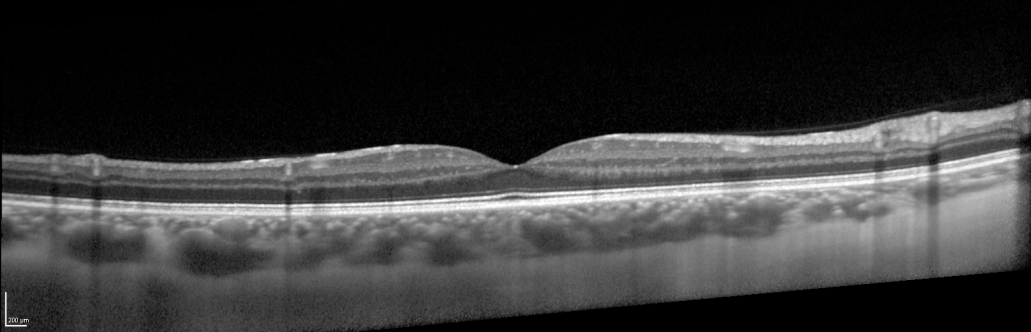
\includegraphics[width=\textwidth]{imagenes/tecnicas/EjemploTecnicasThresholdOriginal.png}}
\end{figure}

\begin{figure}[H]
  \centering \setlength\fboxsep{0pt} \setlength\fboxrule{0.5pt}
  \fbox{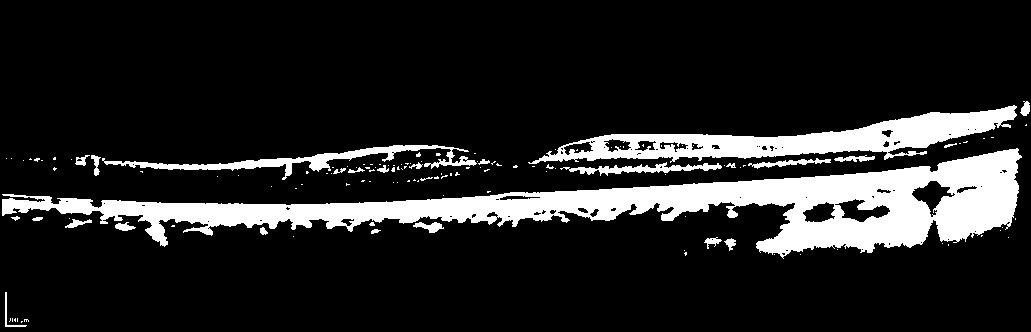
\includegraphics[width=\textwidth]{imagenes/tecnicas/EjemploTecnicasThresholdBinary_127.png}}
  \caption{Treshold Binario}
\end{figure}

\subsubsection{cv2.THRESH\_BINARY\_INV o \emph{Binarización inversa}}
Es la operación contraria al anterior: a los píxeles con un valor
mayor que el valor de umbral se les asigna el valor mínimo, mientras
que los demás adquieren el valor máximo. La expresión es
\begin{equation*}
  destino(x, y) =
  \begin{cases}
    0 & \text{si } entrada(x, y) > umbral \\
    255 & \text{cualquier otro caso}
  \end{cases}
\end{equation*}
Ejemplo para un valor de umbral de $127$ (Arriba original y abajo el
resultado obtenido tras aplicar el filtro):

\begin{figure}[H]
  \caption{Original}
  \centering \setlength\fboxsep{0pt} \setlength\fboxrule{0.5pt}
  \fbox{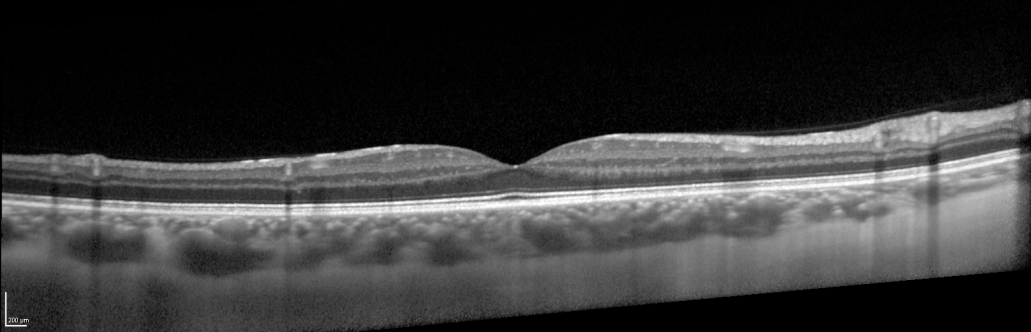
\includegraphics[width=\textwidth]{imagenes/tecnicas/EjemploTecnicasThresholdOriginal.png}}
\end{figure}

\begin{figure}[H]
  \centering \setlength\fboxsep{0pt} \setlength\fboxrule{0.5pt}
  \fbox{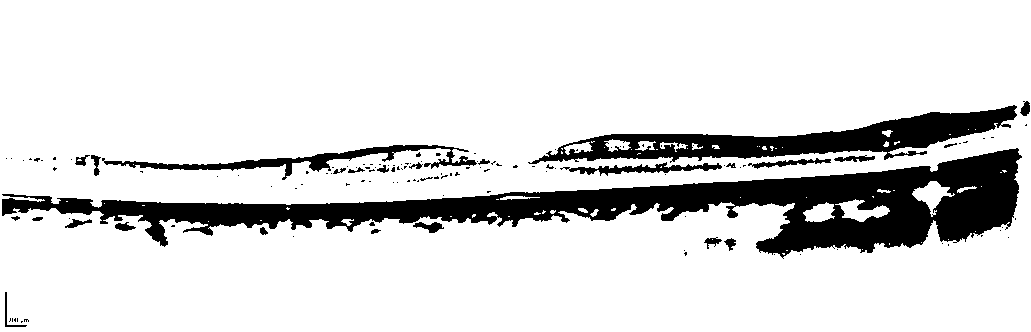
\includegraphics[width=\textwidth]{imagenes/tecnicas/EjemploTecnicasThresholdBinaryInv_127.png}}
  \caption{Threshold Binario Inverso}
\end{figure}


\subsubsection{cv2.THRESH\_TRUNC o \emph{Truncamiento}}
Se trunca el valor de los píxeles de forma que todos los píxeles que
superen el valor de umbral toman dicho valor. En caso contrario se
conserva el valor original. La expresión es
\begin{equation*}
  destino(x, y) =
  \begin{cases}
    umbral & \text{si } entrada(x, y) > umbral \\
    entrada(x, y) & \text{cualquier otro caso}
  \end{cases}
\end{equation*}
Ejemplo para un valor de umbral de $127$ (Arriba original y abajo el
resultado obtenido tras aplicar el filtro):

\begin{figure}[H]
  \caption{Original}
  \centering \setlength\fboxsep{0pt} \setlength\fboxrule{0.5pt}
  \fbox{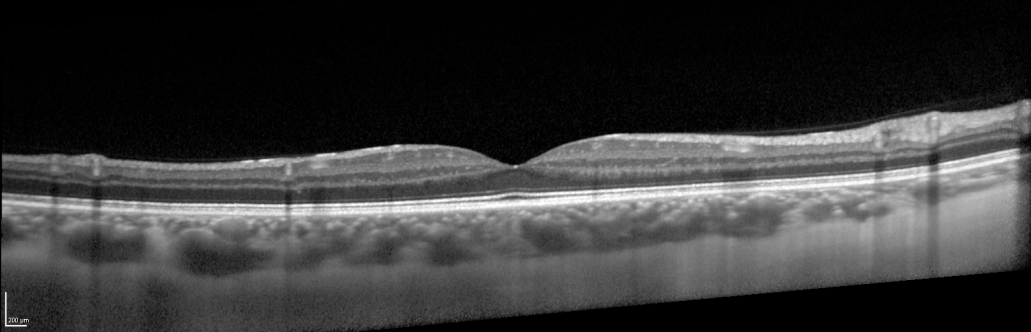
\includegraphics[width=\textwidth]{imagenes/tecnicas/EjemploTecnicasThresholdOriginal.png}}
\end{figure}

\begin{figure}[H]
  \centering \setlength\fboxsep{0pt} \setlength\fboxrule{0.5pt}
  \fbox{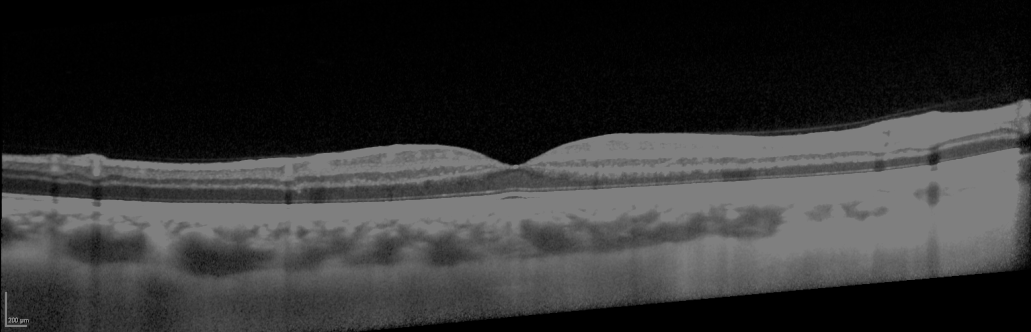
\includegraphics[width=\textwidth]{imagenes/tecnicas/EjemploTecnicasThresholdTrunc_127.png}}
  \caption{Threshold de Truncado}
\end{figure}


\subsubsection{cv2.THRESH\_TOZERO}
Es la operación contraria a la anterior: los píxeles que superen el
valor del umbral conservan su valor original, mientras que en el caso
contrario se les aplica el valor mínimo. La expresión es
\begin{equation*}
  destino(x, y) =
  \begin{cases}
    entrada(x, y) & \text{si } entrada(x, y) > umbral \\
    0 & \text{cualquier otro caso}
  \end{cases}
\end{equation*}
Ejemplo para un valor de umbral de $127$ (Arriba original y abajo el
resultado obtenido tras aplicar el filtro):

\begin{figure}[H]
  \caption{Original}
  \centering \setlength\fboxsep{0pt} \setlength\fboxrule{0.5pt}
  \fbox{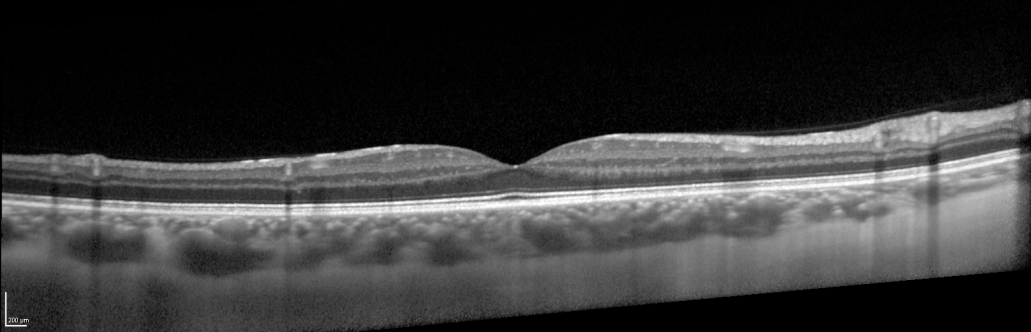
\includegraphics[width=\textwidth]{imagenes/tecnicas/EjemploTecnicasThresholdOriginal.png}}
\end{figure}

\begin{figure}[H]
  \centering \setlength\fboxsep{0pt} \setlength\fboxrule{0.5pt}
  \fbox{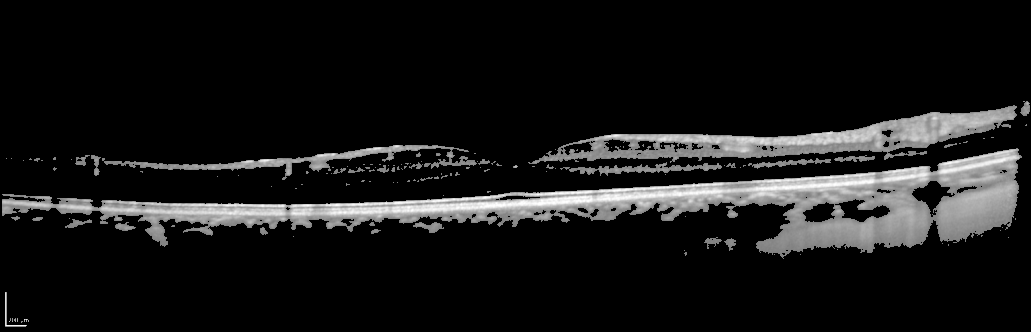
\includegraphics[width=\textwidth]{imagenes/tecnicas/EjemploTecnicasThresholdTo0_127.png}}
  \caption{Threshold to Zero}
\end{figure}

\subsubsection{cv2.THRESH\_TOZERO\_INV}
A los píxeles que superen el valor de umbral se les aplica el valor
mínimo, mientras que en caso contrario conservan el valor original. La
expresión es
\begin{equation*}
  destino(x, y) =
  \begin{cases}
    0  & \text{si } entrada(x, y) > umbral \\
    entrada(x, y) & \text{cualquier otro caso}
  \end{cases}
\end{equation*}
Ejemplo para un valor de umbral de $127$ (Arriba original y abajo el
resultado obtenido tras aplicar el filtro):

\begin{figure}[H]
  \caption{Original}
  \centering \setlength\fboxsep{0pt} \setlength\fboxrule{0.5pt}
  \fbox{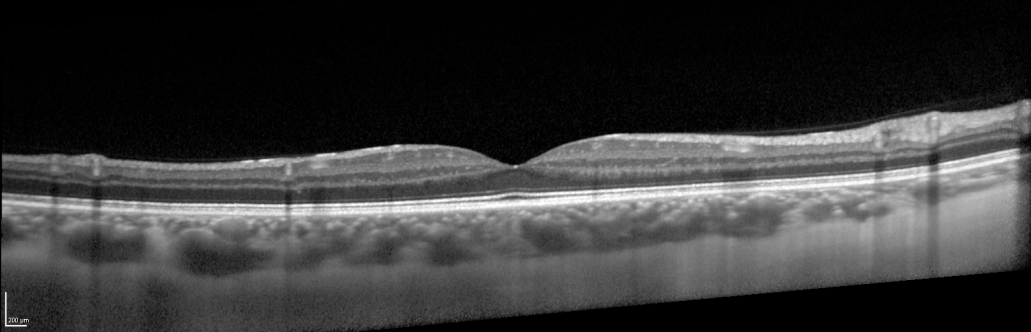
\includegraphics[width=\textwidth]{imagenes/tecnicas/EjemploTecnicasThresholdOriginal.png}}
\end{figure}

\begin{figure}[H]
  \centering \setlength\fboxsep{0pt} \setlength\fboxrule{0.5pt}
  \fbox{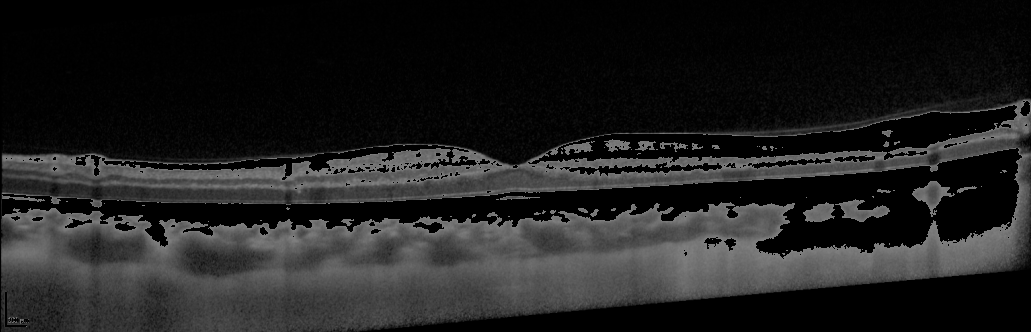
\includegraphics[width=\textwidth]{imagenes/tecnicas/EjemploTecnicasThresholdTo0Inv_127.png}}
  \caption{Threshold to Zero Inverso}
\end{figure}

\subsection{Adaptativos}
En imágenes uniformes aplicar valores umbral globales y fijos suele
ser una buena opción pero para imágenes no uniformes hay que adaptar
dicho valor a cada área de la imagen. Por ello, se aplican las
técnicas siguientes. En ambas, el área a realizar el
\emph{threshold}~\emph{\citep*[6.2 Adaptive
  Thresholding]{fisher1996hypermedia}} depende del tamaño del
\emph{kernel} usado.

\subsubsection{cv2.ADAPTIVE\_THRESH\_MEAN\_C}
El valor de cada píxel se establece por la media de sus vecinos
restándole una constante $C$.

\begin{figure}[H]
  \caption{Original}
  \centering \setlength\fboxsep{0pt} \setlength\fboxrule{0.5pt}
  \fbox{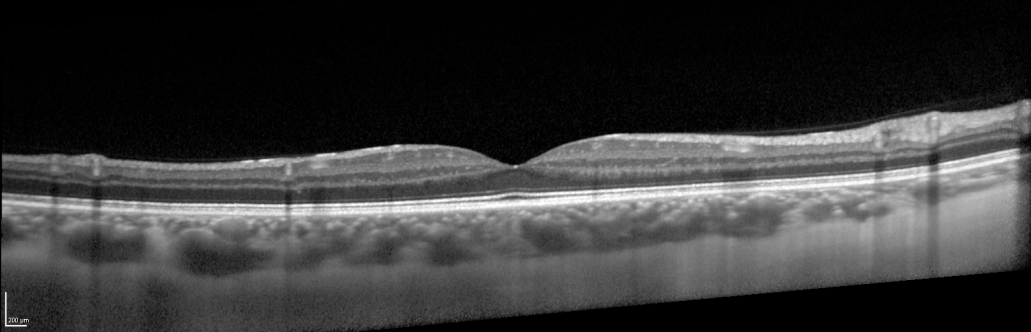
\includegraphics[width=\textwidth]{imagenes/tecnicas/EjemploTecnicasThresholdOriginal.png}}
\end{figure}

\begin{figure}[H]
  \centering \setlength\fboxsep{0pt} \setlength\fboxrule{0.5pt}
  \fbox{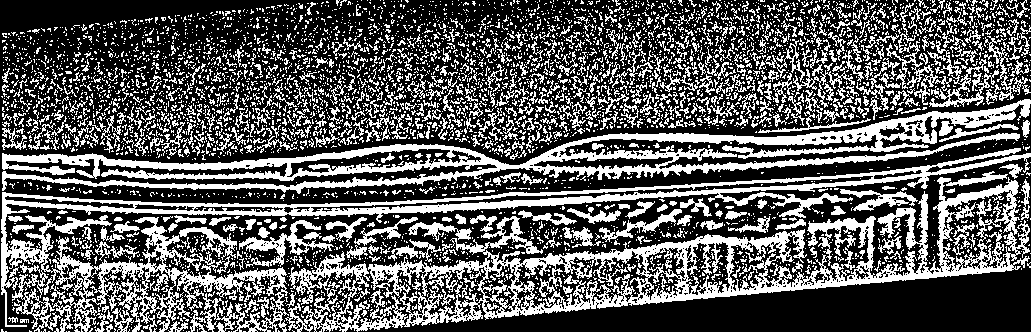
\includegraphics[width=\textwidth]{imagenes/tecnicas/EjemploTecnicasThresholdAdaptiveMeanKernel11Constant2.png}}
  \caption{Mean Adaptive Threshold}
\end{figure}

\subsubsection{cv2.ADAPTIVE\_THRESH\_GAUSSIAN\_C}\label{tecnica:threshold-adaptativo-gauss}
El valor de cada píxel se establece por el resultado de una función
Gaussiana a partir de sus vecinos y restándole una constante $C$.

\begin{figure}[H]
  \caption{Original}
  \centering \setlength\fboxsep{0pt} \setlength\fboxrule{0.5pt}
  \fbox{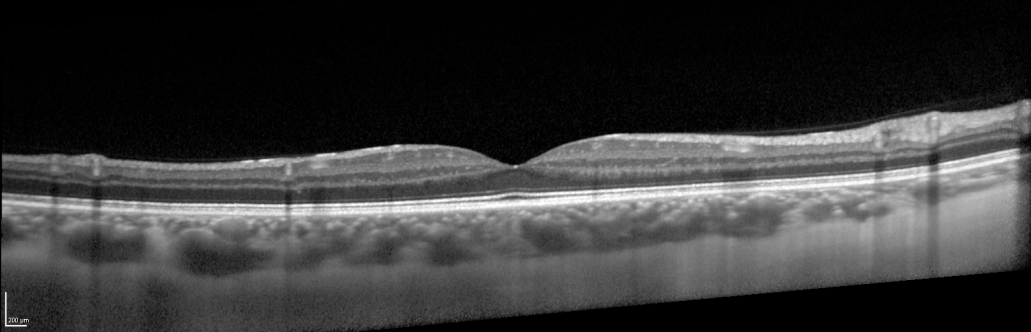
\includegraphics[width=\textwidth]{imagenes/tecnicas/EjemploTecnicasThresholdOriginal.png}}
\end{figure}

\begin{figure}[H]
  \centering \setlength\fboxsep{0pt} \setlength\fboxrule{0.5pt}
  \fbox{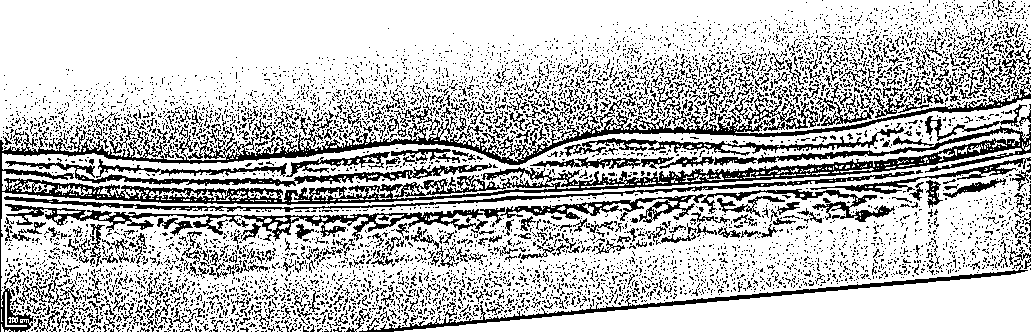
\includegraphics[width=\textwidth]{imagenes/tecnicas/EjemploTecnicasThresholdAdaptiveGaussianKernel11Constant2.png}}
  \caption{Gaussian Adaptive Threshold}
\end{figure}

\subsection{Otsu}\label{tecnica:threshold-otsu}
Este \emph{threshold}\emph{~\citep*[A threshold selection method from
  gray-level histograms]{otsu1975threshold}} calcula el valor umbral a
partir del histograma de la imagen. La precisión de esta técnica
depende de que el histograma sea lo más bimodal posible, en los que
predomina dos columnas.

\begin{figure}[H]
  \caption{Original}
  \centering \setlength\fboxsep{0pt} \setlength\fboxrule{0.5pt}
  \fbox{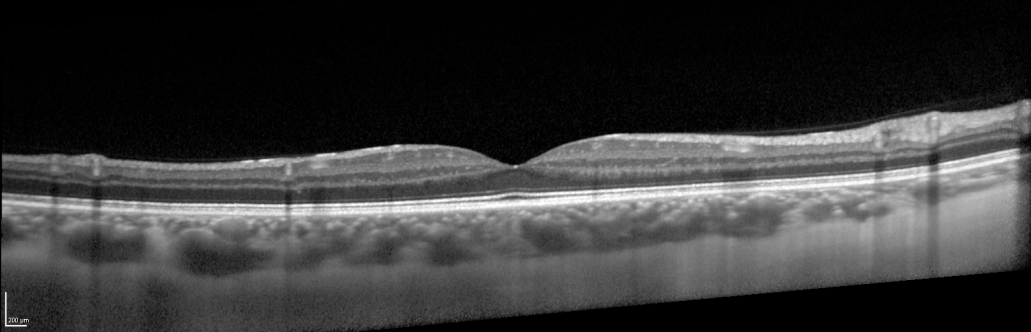
\includegraphics[width=\textwidth]{imagenes/tecnicas/EjemploTecnicasThresholdOriginal.png}}
\end{figure}

\begin{figure}[H]
  \centering \setlength\fboxsep{0pt} \setlength\fboxrule{0.5pt}
  \fbox{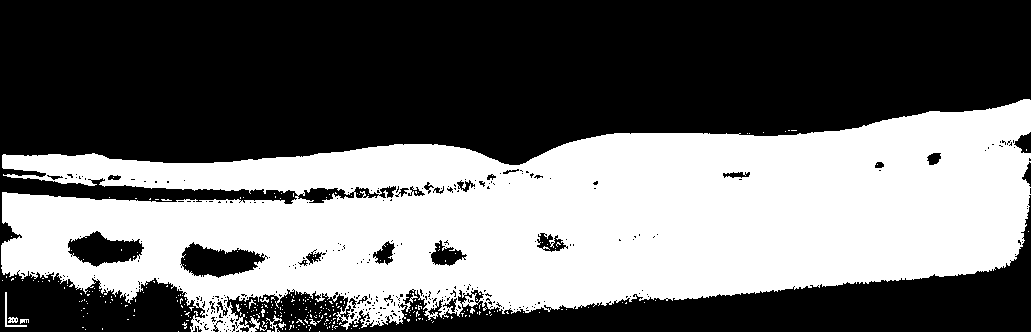
\includegraphics[width=\textwidth]{imagenes/tecnicas/EjemploTecnicasThresholdOtsu.png}}
  \caption{Otsu Threshold}
\end{figure}

\section{Transformaciones geométricas}
Las transformaciones geométricas~\emph{\citep*[Stretch, Shrink, Warp,
  and Rotate]{opencv_book-bib}} son aquellas técnicas en las que se
aplica una matriz o \emph{kernel} de transformación a la imagen
original.
\subsection{Rotación}
Para rotar una imagen desde un ángulo $\theta$ se opera con la siguiente
matriz de transformación.
\begin{equation*}
  M =
  \begin{bmatrix}
    \cos \theta & -\sin \theta \\ \sin \theta & \cos \theta
  \end{bmatrix}
\end{equation*}
\emph{OpenCV} además, facilita una matriz de rotación escalable con
centro ajustable para el punto que se prefiera.
\begin{equation*}
  \begin{bmatrix}
    \alpha & \beta & (1 - \alpha) \cdot centro_x - \beta \cdot centro_y \\
    - \beta & \alpha & \beta \cdot centro_x + (1 - \alpha) \cdot centro_y
  \end{bmatrix}
\end{equation*}
donde:
\begin{center}
  $ \alpha = escala \cdot \cos \theta $
  \\
  $ \beta = escala \cdot \sin \theta $
\end{center}
Para facilitar todavía más la rotación, \emph{OpenCV} proporciona la
función
\begin{center}
  \textbf{cv2.getRotationMatrix2D}(centro, ángulo, escala) \\
  $\downarrow$ \\
  matriz de transformación
\end{center}
Posteriormente hay que aplicar la función de afinidad con la matriz de transformación anterior \\
\begin{center}
  \textbf{cv2.warpAffine}(imagen, matriz, tamaño)\\
  $\downarrow$ \\
  imagen destino
\end{center}

\section{\emph{Blur}}
\emph{Blur}~\emph{\citep*[Smoothing]{opencv_book-bib}}~\emph{\citep*[3.3.1
  Non-linear filtering]{szeliski2010computer}}~\emph{\citep*[4.3 Noise
  Reduction]{toennies2012guide}} o suavizado es una técnica usada con
el objetivo principal de reducir el ruido y los artefactos (contenido
de alta frecuencia) de la imagen, aunque también se usa para disminuir
la resolución. Se basa en aplicar a la imagen un \emph{kernel} de
convolución.
\subsection{Basado en la media}
En el caso de un \emph{blur}, se suman todos los valores de los
píxeles contenidos en la matriz y se divide entre el número de
vecinos. El \emph{kernel} a aplicar es el siguiente
\begin{equation*}
  K = \frac{1}{n}
  \begin{bmatrix}
    1_{11} & 1_{12} & \cdots & 1_{1n} \\
    1_{21} & 1_{22} & \cdots & 1_{2n} \\
    \vdots & \vdots & \ddots & \vdots \\
    1_{n1} & 1_{n2} & \cdots & 1_{nn} \\
  \end{bmatrix}
  \text{siendo \emph{n} un número impar}
\end{equation*}

A modo de ejemplo, el \emph{kernel} de dimensión $3\times3$ es
\begin{equation*}
  K = \frac{1}{9}
  \begin{bmatrix}
    1 & 1 & 1 \\
    1 & 1 & 1 \\
    1 & 1 & 1 \\
  \end{bmatrix}
\end{equation*}
\subsection{Basado en una función Gaussiana}
Esta técnica es la que mejor resultados suele dar, especialmente si se
utiliza para reducir el ruido generado por un \emph{kernel
  Gaussiano}. Cabe destacar que al aplicar este método puede dar como
resultado valores de píxeles que no estuvieran en la imagen
original. Este \emph{Blur} es el menos eficiente de todos pero
\emph{OpenCV} lo optimiza para las sigmas $\sigma_x$ y $\sigma_y$
predeterminadas de los \emph{kernels} de $3\times3$, $5\times5$ y
$7\times7$. Debido a esto, sólo mostraremos como se
generan estas sigmas predeterminas y un ejemplo con ellas.\\
\emph{OpenCV} obliga a introducir $\sigma_x$ y en el caso de que este sea
$0$, se determinan ambos sigmas a partir del tamaño del \emph{kernel}
introducido mediante las fórmulas siguientes:
\begin{equation*}
  \hspace{0.25cm}\sigma_x = \left(\frac{n_x}{2} - 1 \right) \cdot 0,30 + 0,80 \hspace{0.5cm} n_x = \text{anchura del \emph{kernel}}
\end{equation*}
\begin{equation*}
  \sigma_y = \left(\frac{n_y}{2} - 1 \right) \cdot 0,30 + 0,80 \hspace{0.5cm} n_y = \text{altura del \emph{kernel}}
\end{equation*}
Y la función \emph{Gaussiana} en la que se aplican:
\begin{equation*}
  Gaussiana(x, y) = \frac{1}{\sqrt{2 \pi \sigma^{2}}}e^{- \frac{x^{2}+y^{2}}{2\sigma^{2}}}
\end{equation*}
En el siguiente ejemplo se aplica un Blur basado en una función
Gaussiana con \emph{kernel} de $23 \times 23$, a partir del cual se
calculan las \emph{sigmas}:

\begin{figure}[H]
  \caption{Original}
  \centering \setlength\fboxsep{0pt} \setlength\fboxrule{0.5pt}
  \fbox{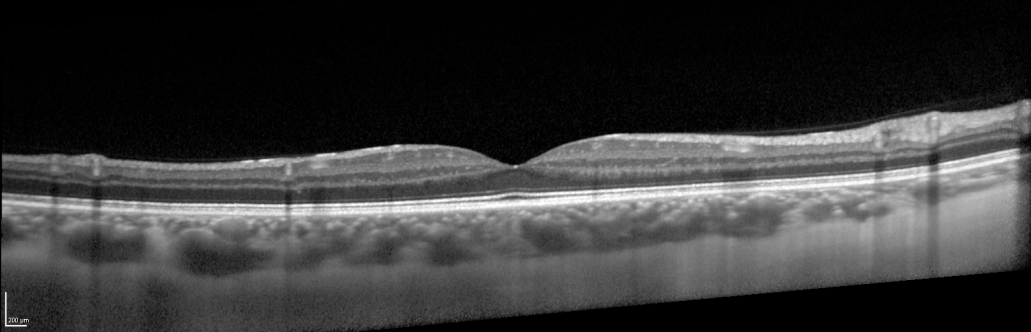
\includegraphics[width=\textwidth]{imagenes/tecnicas/EjemploTecnicasThresholdOriginal.png}}
\end{figure}

\begin{figure}[H]
  \centering \setlength\fboxsep{0pt} \setlength\fboxrule{0.5pt}
  \fbox{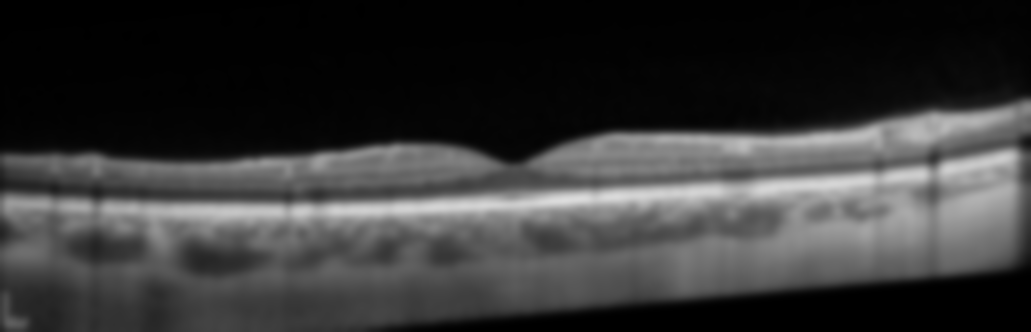
\includegraphics[width=\textwidth]{imagenes/tecnicas/EjemploTecnicasBlurGaussian23x23.png}}
  \caption{Gaussian Blur}
\end{figure}


\subsection{Basado en la mediana}\label{tecnica:blur-median}
En el caso de un \emph{median Blur} y como oposición al \emph{Blur},
que se basa en la media, el \emph{median Blur} calcula el valor
del píxel central mediante la mediana de los píxeles colindantes. \\
Esta técnica es muy útil para reducir el ruido granulado de la imagen.\\
En el siguiente ejemplo se muestra un ejemplo aplicando un
\emph{kernel} de tamaño $23$:

\begin{figure}[H]
  \caption{Original}
  \centering \setlength\fboxsep{0pt} \setlength\fboxrule{0.5pt}
  \fbox{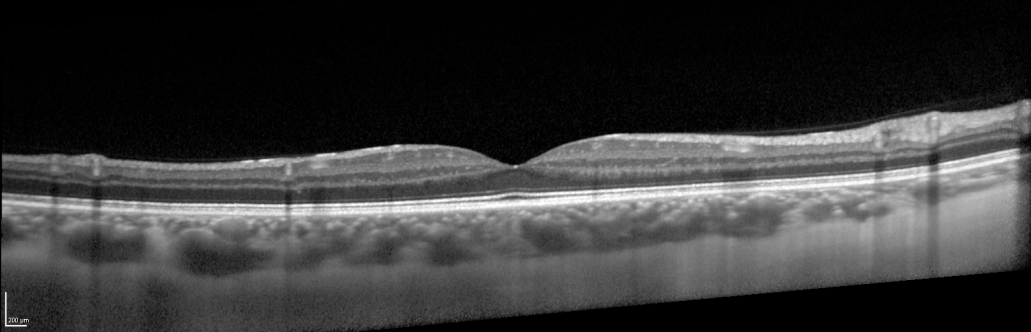
\includegraphics[width=\textwidth]{imagenes/tecnicas/EjemploTecnicasThresholdOriginal.png}}
\end{figure}

\begin{figure}[H]
  \centering \setlength\fboxsep{0pt} \setlength\fboxrule{0.5pt}
  \fbox{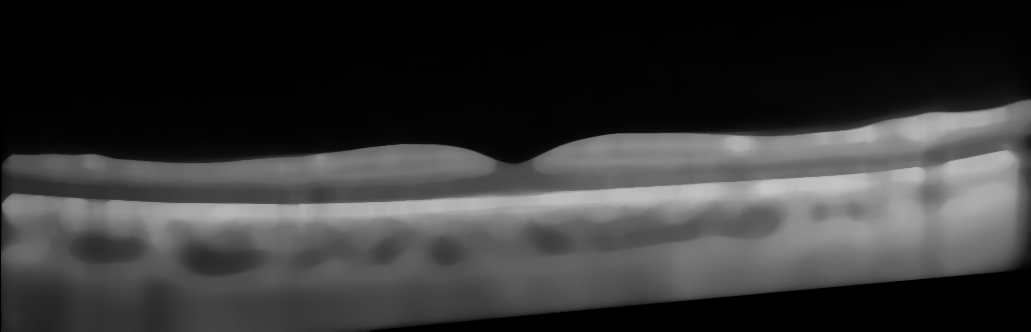
\includegraphics[width=\textwidth]{imagenes/tecnicas/EjemploTecnicasBlurMedian23.png}}
  \caption{Median Blur}
\end{figure}

\section{Transformaciones morfológicas}
Las operaciones de transformación morfológicas~\emph{\citep*[9
  Morphology]{fisher1996hypermedia}}~\emph{\citep*[Image
  Morphology]{opencv_book-bib}} se aplican sobre la forma de la
imagen. Se suelen usar para reducir el ruido, aislar o juntar
elementos. El \emph{kernel} aplicado a la imagen define el
resultado de la operación. \\
Normalmente, este tipo de operaciones se realizan posteriormente a una
operación de \emph{threshold} por lo que para entender mejor la
operación supondremos que la imagen está \emph{binarizada} (píxeles
únicamente blancos o negros). \\
A diferencia de los \emph{kernel} de convolución, los \emph{kernel}
morfológicos no necesitan ser de dimensión cuadrada ni contener
valores numéricos porque se utilizan como referencia para indicar las
posiciones de los píxeles.

\subsection{\emph{Erosion}}
Es una técnica que usa un \emph{kernel} a modo de máscara, sustituye
el píxel central por el \emph{mínimo local} de sus vecinos. Si algún
vecino es un píxel negro, automáticamente el píxel central se
convertirá en negro. El nombre procede del efecto que produce en una
imagen un artefacto blanco sobre fondo negro dando la sensación de
reducción del artefacto y reduciendo sus salientes. La fórmula es:
\begin{equation*}
  erode(x, y) = \min_{\substack{(x', y' \in \; kernel)}} imagen(x + x', y + y')
\end{equation*}
El siguiente ejemplo muestra el efecto de someter una imagen a una
operación de \emph{Erosion} con un \emph{kernel} de $5 \times 5$ todo
de unos:

\begin{figure}[H]
  \caption{Original}
  \centering \setlength\fboxsep{0pt} \setlength\fboxrule{0.5pt}
  \fbox{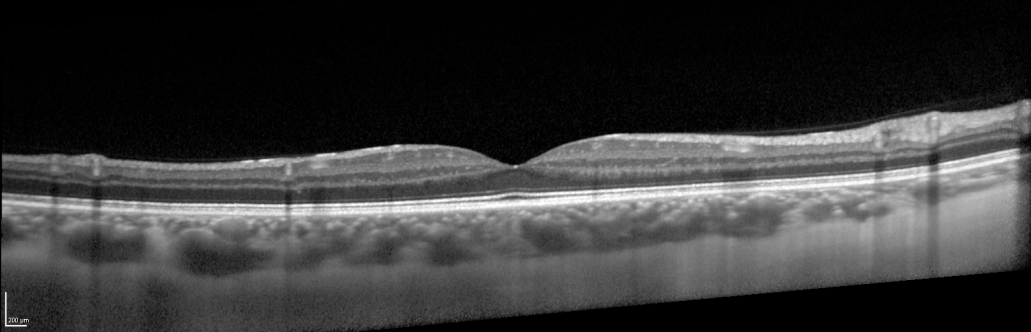
\includegraphics[width=\textwidth]{imagenes/tecnicas/EjemploTecnicasThresholdOriginal.png}}
\end{figure}

\begin{figure}[H]
  \centering \setlength\fboxsep{0pt} \setlength\fboxrule{0.5pt}
  \fbox{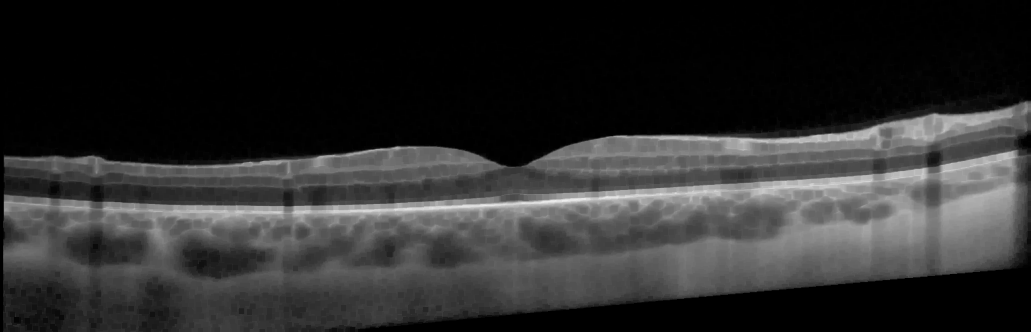
\includegraphics[width=\textwidth]{imagenes/tecnicas/EjemploTecnicasErosion.png}}
  \caption{Erosion}
\end{figure}


\subsection{\emph{Dilation}}\label{tecnica:dilation}
Es la técnica inversa a \emph{Erosion}, de la misma manera un
\emph{kernel} a modo de máscara sustituye el píxel central por el
\emph{máximo local}. Si alguno de sus vecinos es un píxel blanco, el
central automáticamente se convertirá en blanco. Igualmente, el nombre
procede del efecto que produce en una imagen con un artefacto blanco
sobre fondo negro dando la sensación de la dilatación del artefacto y
reduciendo sus concavidades. La fórmula es:
\begin{equation*}
  dilate(x, y) = \max_{\substack{(x', y' \in \;kernel)}} imagen(x + x', y + y')
\end{equation*}
El siguiente ejemplo muestra el efecto de someter una imagen a una
operación de \emph{Dilation} con un \emph{kernel} de $5 \times 5$ todo
de unos:

\begin{figure}[H]
  \caption{Original}
  \centering \setlength\fboxsep{0pt} \setlength\fboxrule{0.5pt}
  \fbox{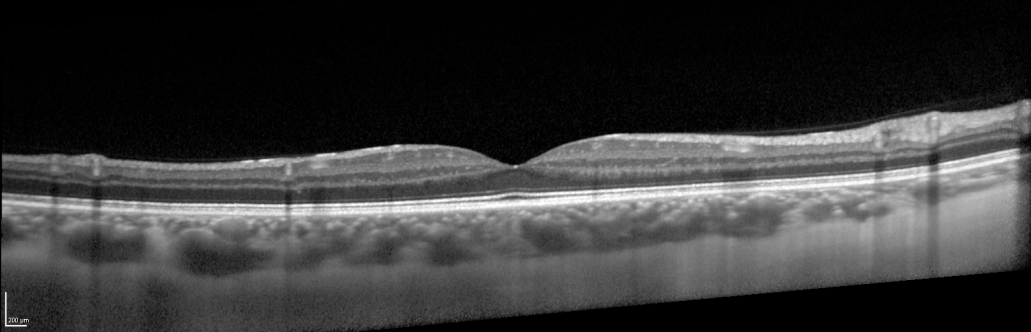
\includegraphics[width=\textwidth]{imagenes/tecnicas/EjemploTecnicasThresholdOriginal.png}}
\end{figure}

\begin{figure}[H]
  \centering \setlength\fboxsep{0pt} \setlength\fboxrule{0.5pt}
  \fbox{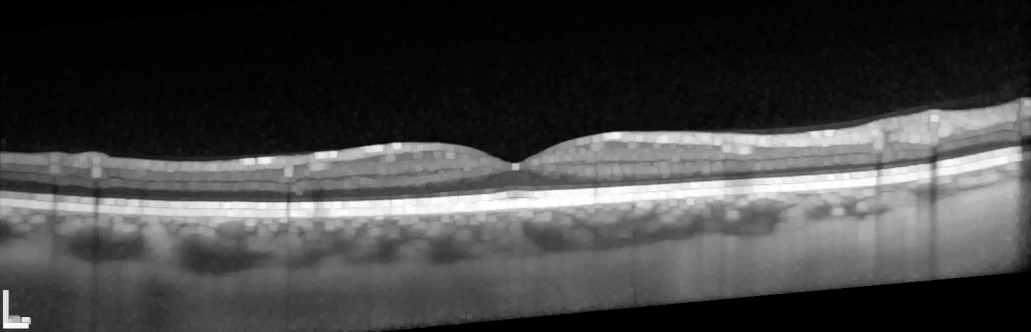
\includegraphics[width=\textwidth]{imagenes/tecnicas/EjemploTecnicasDilation.png}}
  \caption{Dilation}
\end{figure}

\subsection{\emph{Opening}}
La técnica de \emph{Opening} consiste en la realización de un
\emph{Erode} seguido de un \emph{Dilate}. Se utiliza para la
eliminación de ruido granulado alrededor del artefacto.\\
En el siguiente ejemplo se somete a la imagen a un \emph{Opening} con
\emph{kernel} de tamaño $5$:

\begin{figure}[H]
  \caption{Original}
  \centering \setlength\fboxsep{0pt} \setlength\fboxrule{0.5pt}
  \fbox{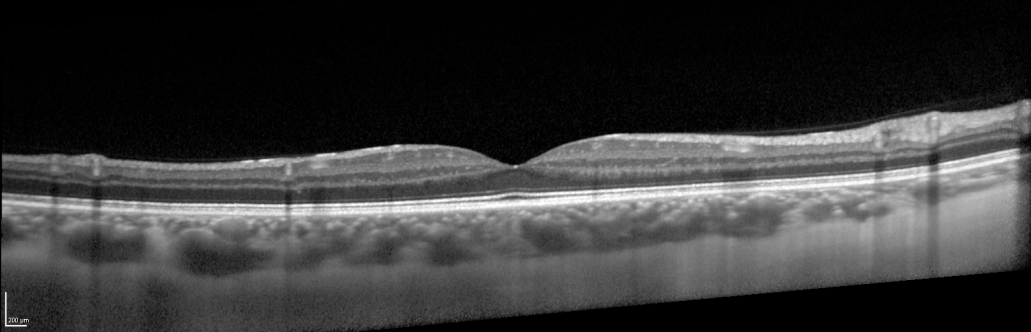
\includegraphics[width=\textwidth]{imagenes/tecnicas/EjemploTecnicasThresholdOriginal.png}}
\end{figure}

\begin{figure}[H]
  \centering \setlength\fboxsep{0pt} \setlength\fboxrule{0.5pt}
  \fbox{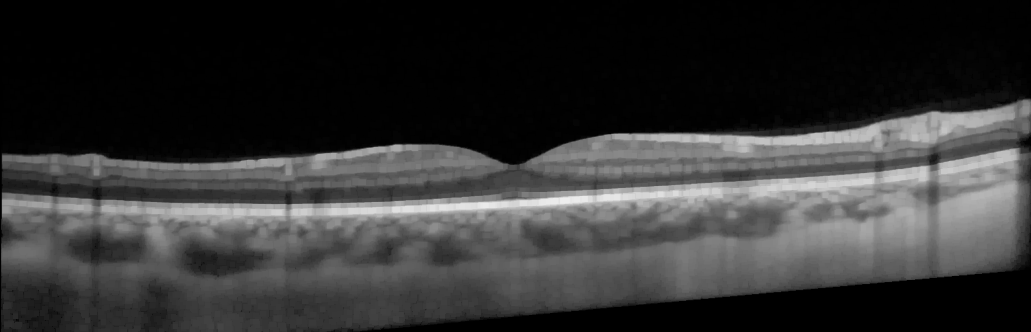
\includegraphics[width=\textwidth]{imagenes/tecnicas/EjemploTecnicasOpening5.png}}
  \caption{Opening}
\end{figure}

\subsection{\emph{Closing}}
La técnica de \emph{Closing} consiste en la realización de un
\emph{Dilate} seguido de un \emph{Erode}. Se utiliza para la
eliminación de ruido granulado situado en el interior del
artefacto. \\
En el siguiente ejemplo se somete a la imagen a un \emph{Closing} con
\emph{kernel} de tamaño $5$:

\begin{figure}[H]
  \caption{Original}
  \centering \setlength\fboxsep{0pt} \setlength\fboxrule{0.5pt}
  \fbox{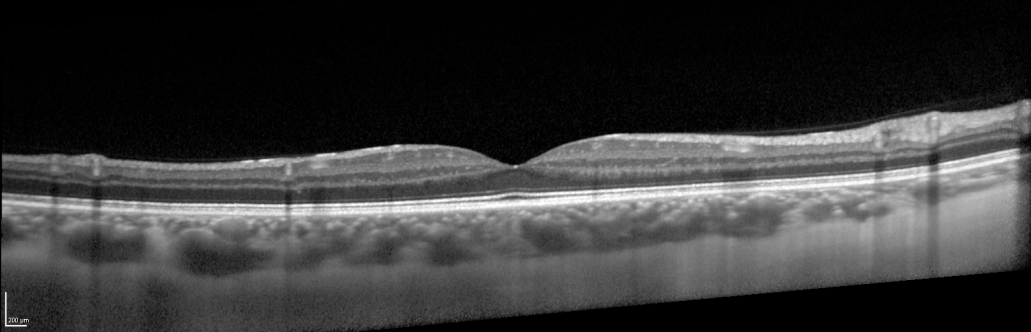
\includegraphics[width=\textwidth]{imagenes/tecnicas/EjemploTecnicasThresholdOriginal.png}}
\end{figure}

\begin{figure}[H]
  \centering \setlength\fboxsep{0pt} \setlength\fboxrule{0.5pt}
  \fbox{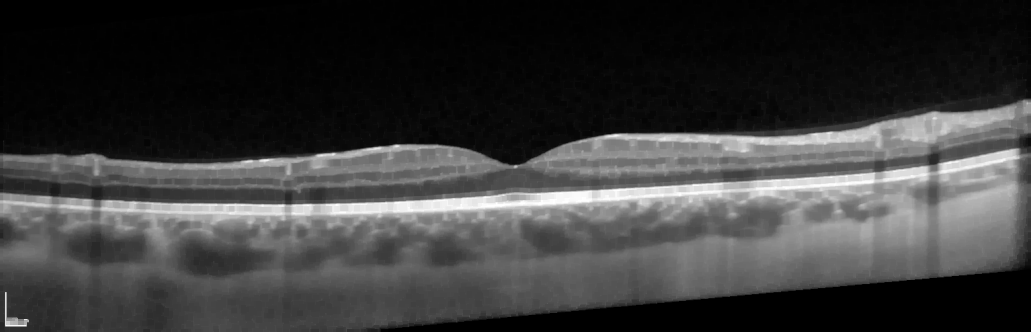
\includegraphics[width=\textwidth]{imagenes/tecnicas/EjemploTecnicasClosing5.png}}
  \caption{Opening}
\end{figure}

\subsection{Gradiente morfológico}
Es la diferencia entre la operación \emph{Dilation} y la operación
\emph{Erode} de la imagen. Se utiliza para marcar el perímetro o borde
del artefacto. La expresión es:
\begin{equation*}
  gradiente(imagen) = dilate(imagen) - erode(imagen)
\end{equation*}

\section{Gradientes}
El cálculo de gradientes o bordes \emph{\citep*[11. Feature
  Detectors]{fisher1996hypermedia}} \emph{\citep*[Gradients and Sobel
  Derivatives]{opencv_book-bib}} \emph{\citep*[5.1 Edge
  Tracking]{toennies2012guide}} se realiza mediante la convolución de
derivadas parciales del estilo:
\begin{equation*}
  \frac{\delta^{2}}{\delta x \delta y}
\end{equation*}
Por simplificación y eficiencia nos centraremos en describir sus
aproximaciones, más fáciles de entender. \\
El origen de los números de los \emph{kernels} se basa en el siguiente
proceso:\\
Una imagen se puede representar como una función de una señal continua
y discreta. Nos centraremos en ver el proceso con una fila de píxeles
de la imagen. Un borde es un cambio de color que en la función está
representado como un cambio de valor entre una posición y
otra. Matemáticamente, la manera de medir cuánto cambia entre un punto
,por ejemplo $x$, y otro muy próximo, $x + \delta x$, se realiza
mediante la
derivación.\\
La fórmula para derivar una imagen $I$ que sólo contenga una fila de
píxeles es la siguiente:
\begin{equation*}
  I'_x(x) = \lim_{\delta x \to 0}\frac{I(x+\delta x) - I(x)}{\delta x}
\end{equation*}
Como sólo se pueden computar valores discretos, el punto de la función
más cercano a $0$ es $\delta x = 1$. Esto aproxima la derivada a
\begin{equation*}
  I_x'(x) \approx I(x + 1) - I(x)
\end{equation*}
Si extraemos los coeficientes de las imágenes a un \emph{kernel}, el
resultado es:
\begin{equation*}
  kernel = \begin{bmatrix}
    1 & -1
  \end{bmatrix}
\end{equation*}
Nótese que la suma de todos los coeficientes siempre será $0$. Para
alargar el \emph{kernel} y abarcar más píxeles, por ejemplo tres, se
procede a introducir $0$ entre medias dando lugar a
$\begin{bmatrix} 1 & 0 & -1 \end{bmatrix}$ \\
Al realizar la primera derivada, nos encontramos que para interpretar
el gradiente tiene que ser un máximo local y suficientemente alto para
distinguirlo. Por lo que si aplicamos la segunda derivada suavizamos
el gradiente y obtenemos, de manera precisa, el máximo local, porque
toma el valor $0$ en el eje de abcisas. Si alargamos el \emph{kernel}
en los ejes $x, y$ obtendremos el \emph{kernel}
\emph{Sobel} que se explicará con detenimiento en el siguiente apartado. \\
La segunda derivada viene dada por:
\begin{equation*}
  I''(x) = \lim_{\delta x \to 0}\frac{I'(x+\delta x) - I'(x)}{\delta x}
\end{equation*}
Si aproximamos como la vez anterior $\delta x = 1$ obtenemos
\begin{equation*}
  I_x''(x) \approx I'(x + 1) - I'(x)
\end{equation*}
Como ya hemos aproximado la primera derivada:
\begin{equation*}
  I'(x) \approx I(x + 1) - I(x)
\end{equation*}
Podemos aplicarla a la segunda
\begin{equation*}
  I''(x) \approx \underbrace{I'(x + 1)}_{I(x + 2) - I(x + 1)} - \underbrace{I'(x)}_{I(x + 1) - I(x)}
\end{equation*}
Dando como resultado:
\begin{equation*}
  I''(x) \approx I(x) - 2I(x + 1) + I(x + 2)
\end{equation*}
Y al \emph{kernel} $\begin{bmatrix} 1 & -2 & 1 \end{bmatrix}$ que si
se expande en dos direcciones del espacio se obtiene el \emph{kernel}
siguiente.
\subsection{Sobel}
Como el operador \emph{Sobel} \emph{\citep*[History and definition of
  the sobel operator]{sobel2014history}} está definido en un espacio
discreto no es exactamente una derivada, representa un polinomio y la
segunda derivada, una función parabólica. Por esta razón, cuanto más
grande y más píxeles abarque el \emph{kernel} mejor aproximación se
obtiene y más tolerancia al ruido.
\begin{center}
  $ G_x = \begin{bmatrix}
    -1 & 0 & +1 \\
    -2 & 0 & +2 \\
    -1 & 0 & +1 \\
  \end{bmatrix}
  \hspace{0.5cm} \text{ y } \hspace{0.5cm} G_y = \begin{bmatrix}
    -1 & -2 & -1 \\
    0 & 0 & 0 \\
    +1 & +2 & +1 \\
  \end{bmatrix}
  $
  \\[0.5cm]
  $G = \sqrt{G_x\,^2 + G_y\,{2}}$
  \\[0.5cm]
  $\Theta= \arctan\left(\frac{G_y}{G_x} \right)$
\end{center}
La aproximación con el \emph{kernel} se hace de la siguiente manera:
\begin{equation*}
  Sobel(imagen) = \frac{\delta^{orden_x + orden_y} imagen}{\delta x^{orden_x} \delta
    y^{orden_y}} \text{ siendo el orden de derivación } orden_y \text{ y } orden_y > 0
\end{equation*}

\begin{figure}[H]
  \caption{Original}
  \centering \setlength\fboxsep{0pt} \setlength\fboxrule{0.5pt}
  \fbox{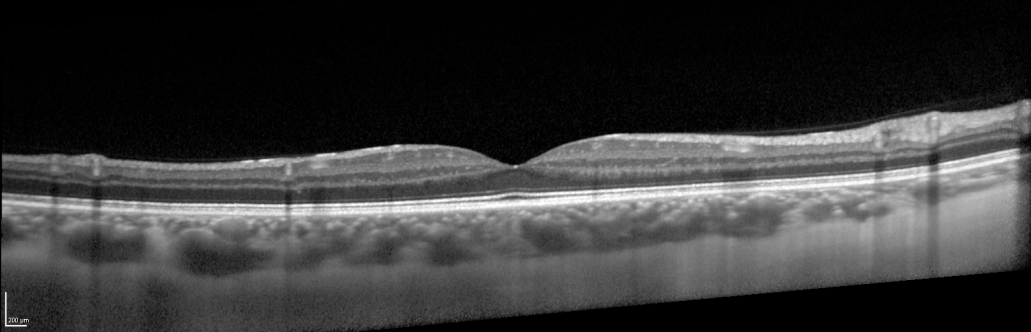
\includegraphics[width=\textwidth]{imagenes/tecnicas/EjemploTecnicasThresholdOriginal.png}}
\end{figure}

\begin{figure}[H]
  \centering \setlength\fboxsep{0pt} \setlength\fboxrule{0.5pt}
  \fbox{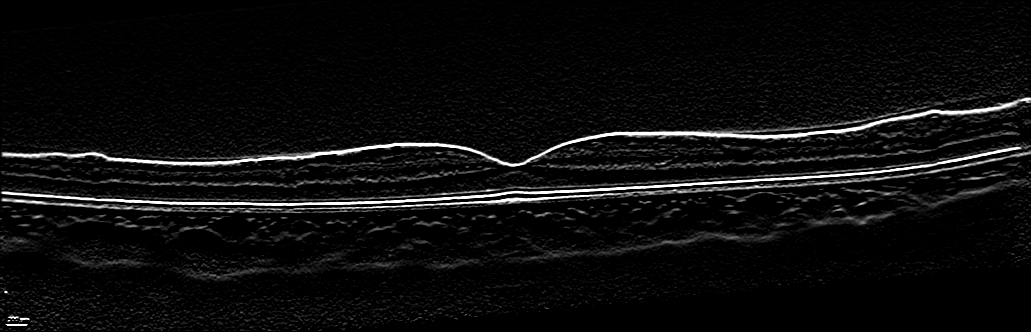
\includegraphics[width=\textwidth]{imagenes/tecnicas/EjemploTecnicasSobel.png}}
  \caption{Sobel}
\end{figure}

\subsection{Scharr}
El operador \emph{Scharr} se utiliza como el sustituto del operador
\emph{Sobel} cuando es necesario aplicar \emph{kernels} pequeños,
especialmente de tamaño $3 \times 3$, en los cuales al tener tan pocos
píxeles, los bordes no suelen estar posicionados sobre los ejes $x$ e
$y$ como en la superficie de los \emph{kernel} de gran tamaño por lo
que la aproximación de \emph{Sobel} es bastante inexacta con los
gradientes en forma de ángulo.
\begin{center}
  $ G_x = \begin{bmatrix}
    +3 & 0 & -3 \\
    +10 & 0 & -10 \\
    +3 & 0 & -3 \\
  \end{bmatrix}
  \hspace{0.5cm} \text{ y } \hspace{0.5cm} G_y = \begin{bmatrix}
    +3 & +10 & +10 \\
    0 & 0 & 0 \\
    -3 & -10 & -10 \\
  \end{bmatrix}
  $
\end{center}

\begin{figure}[H]
  \caption{Original}
  \centering \setlength\fboxsep{0pt} \setlength\fboxrule{0.5pt}
  \fbox{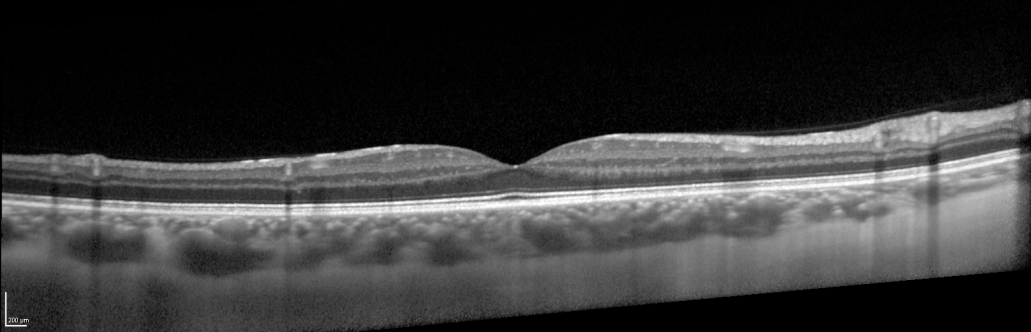
\includegraphics[width=\textwidth]{imagenes/tecnicas/EjemploTecnicasThresholdOriginal.png}}
\end{figure}

\begin{figure}[H]
  \centering \setlength\fboxsep{0pt} \setlength\fboxrule{0.5pt}
  \fbox{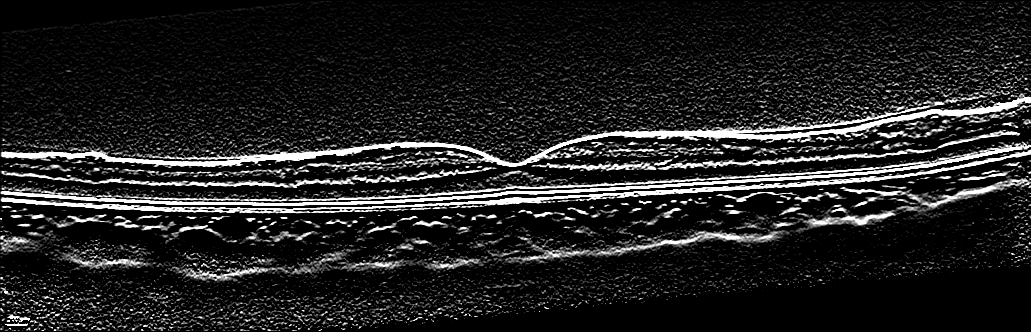
\includegraphics[width=\textwidth]{imagenes/tecnicas/EjemploTecnicasScharr.png}}
  \caption{Scharr}
\end{figure}

\subsection{Laplaciano}
El operador \emph{Laplaciano} se define como la segunda derivada del
operador \emph{Sobel} de la siguiente manera:
\begin{equation*}
  Laplaciana(imagen) = \frac{\delta^{2} imagen}{\delta x^{2}} + \frac{\delta^{2} imagen}{\delta y^{2}}
\end{equation*}
Por motivos de eficiencia, se aproxima con el \emph{kernel} siguiente
\begin{center}
  $ kernel = \begin{bmatrix}
    0 & +1 & 0 \\
    +1 & -4 & +1 \\
    0 & +1 & 0 \\
  \end{bmatrix}
  $
\end{center}

\begin{figure}[H]
  \caption{Original}
  \centering \setlength\fboxsep{0pt} \setlength\fboxrule{0.5pt}
  \fbox{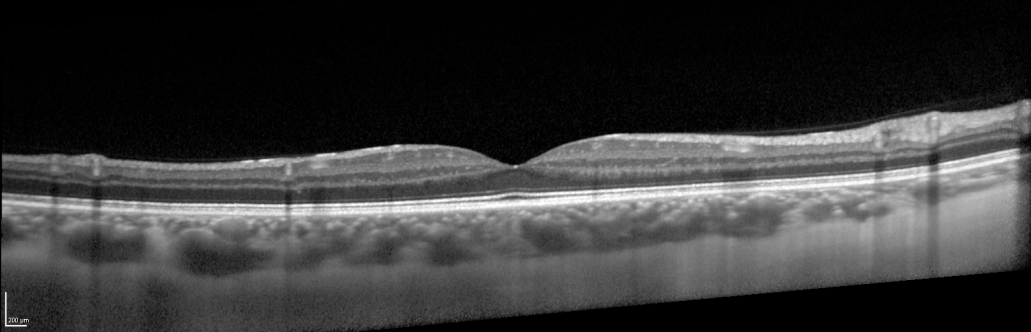
\includegraphics[width=\textwidth]{imagenes/tecnicas/EjemploTecnicasThresholdOriginal.png}}
\end{figure}

\begin{figure}[H]
  \centering \setlength\fboxsep{0pt} \setlength\fboxrule{0.5pt}
  \fbox{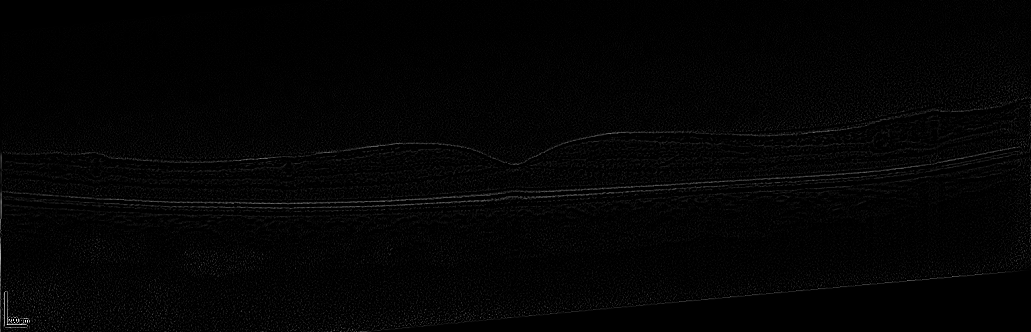
\includegraphics[width=\textwidth]{imagenes/tecnicas/EjemploTecnicasLaplacian.png}}
  \caption{Laplaciano}
\end{figure}

\section{Algoritmo \emph{Canny}}\label{tecnica:canny}
El \emph{Canny} \emph{\citep*[A computational approach to edge
  detection]{canny1986computational}}
\emph{\citep*[Canny]{opencv_book-bib}} \emph{\citep*[5.1 Edge
  Tracking]{toennies2012guide}} es un algoritmo de detección de bordes
conocido como el \emph{detector óptimo} con la función de satisfacer
tres criterios principales:
\begin{itemize}
\item Bajo índice de error.
\item Minimización de la distancia entre los bordes detectados y los
  reales.
\item Un único detector por borde.
\end{itemize}
Para ello lo primero que hace es descartar el ruido usando el filtro
Gaussiano.
El \emph{kernel} usado para este filtro no es fijo.\\
Luego encuentra la intensidad del gradiente de la imagen con
procedimiento similar al Sobel con las mismas máscaras de convolución,
fuerza del gradiente y dirección.\\
Posteriormente, se suprimen los píxeles que no se consideran parte del
borde de forma que solo queden unas finas líneas. Estas líneas son los posibles bordes.\\
Por último, se usan dos \emph{thresholds}, uno alto y uno bajo: Si el
gradiente del píxel es mayor que el threshold alto, el píxel formará
parte del borde; si el gradiente del píxel es menor que el threshold
bajo, no se tendrá en cuenta; en caso de que el gradiente del píxel
esté entre ambos \emph{thresholds} se considerará solo si está
contiguo a un píxel cuyo gradiente sea superior al threshold alto.\\
El siguiente ejemplo muestra el resultado de aplicar \emph{Canny} a
una imagen:

\begin{figure}[H]
  \caption{Original}
  \centering \setlength\fboxsep{0pt} \setlength\fboxrule{0.5pt}
  \fbox{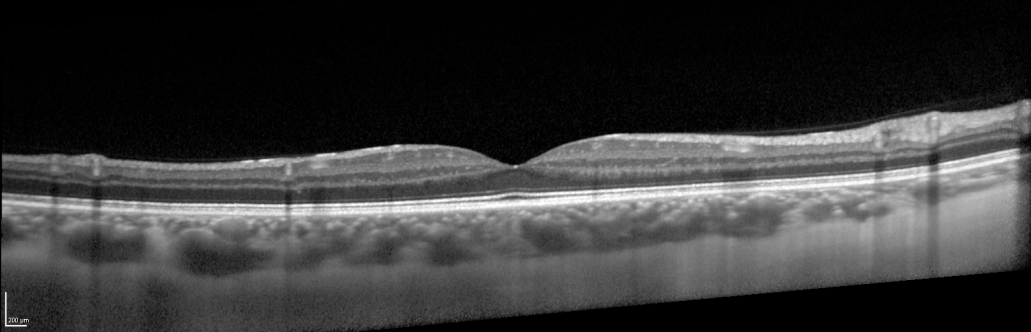
\includegraphics[width=\textwidth]{imagenes/tecnicas/EjemploTecnicasThresholdOriginal.png}}
\end{figure}

\begin{figure}[H]
  \centering \setlength\fboxsep{0pt} \setlength\fboxrule{0.5pt}
  \fbox{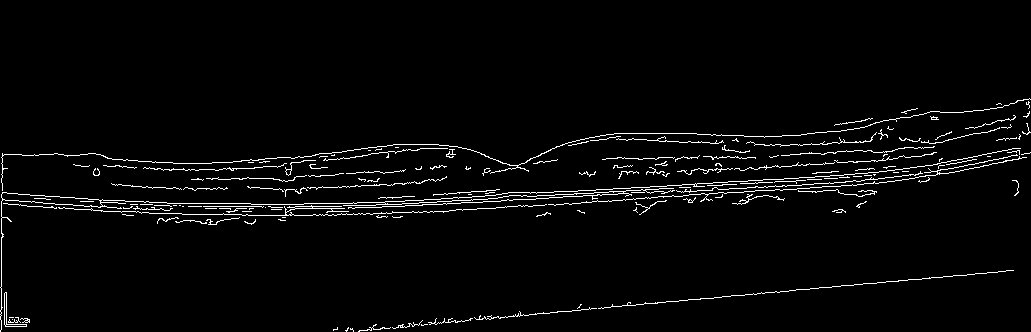
\includegraphics[width=\textwidth]{imagenes/tecnicas/EjemploTecnicasCanny.png}}
  \caption{Canny}
\end{figure}

\section{Transformada de \emph{Hough}}\label{tecnica:hough}
La transformada de \emph{Hough} \emph{\citep*[Use of the hough
  trasformtion to detect lines and curves in pictures]{hart1971use}}
\emph{\citep*[4.3.2 Hough transforms]{szeliski2010computer}}
\emph{\citep*[5.2 Hough Transform]{toennies2012guide}} es una técnica
que se aplica para encontrar formas en una imagen \emph{binarizada} o
tras haber aplicado un algoritmo de detección de bordes y contornos
como el \emph{Canny}, incluso aunque haya ruido, siempre que se puedan
expresar matemáticamente como líneas rectas y curvas. Nos centraremos
sólo en explicar con rectas.
\subsection{Rectas}
Cualquier punto obtenido de una imagen puede formar parte de una línea
recta. Representamos una recta de manera simplificada como
\begin{equation*}
  y = mx + c
\end{equation*}
O mejor, de forma paramétrica porque al pasar infinitas rectas por un
punto lo más sencillo es limitar a un rango de ángulos.
\begin{equation*}
  \rho = x \cos \theta + y \sin \theta
\end{equation*}
donde $\rho$ es la distancia perpendicular a la recta desde el origen y
$\theta$ el ángulo que forman la recta de la distancia con el
origen. En \emph{OpenCV} el origen está situado en la parte superior
izquierda. Si la recta a dibujar corta al eje de abcisas con un valor
positivo el ángulo $\theta$ es menor que $180º$ y el valor de $\rho$
es positivo. Por el contrario, si corta al eje de abcisas por un valor
negativo, el ángulo $\theta$ es mayor de $180º$ y $\rho$ es
negativo. Los casos extremos son las líneas verticales $0º$ y
horizontales $90º$.\\
Por claridad, imaginemos sólo dos puntos por los que queremos trazar
una recta. Para ello, trazaremos tantas rectas como $\theta$
determinemos por cada punto, almacenando de cada uno su $\theta$ y su
$\rho$. Con estos pares, se construye una gráfica donde el eje $y$ de
ordenadas sea $\rho$ y el eje $x$ de abcisas sea $\theta$. Cada punto
genera una curva y en el punto de intersección de las dos encontramos
la $\theta$ y $\rho$ de la recta que pasa por los dos puntos. Por
supuesto, \emph{OpenCV} no calcula la gráfica sino que guarda los
pares y acumula el número de apariciones de cada uno y finalmente
devuelve el máximo local.

\section{Contornos}\label{tecnica:contornos}
Un contorno es una línea curva formada por la únión de puntos que
tienen el mismo color o intensidad. La detección de contornos
\emph{\citep*[Contours in OpenCV]{opencv_tutorial-bib}}
\emph{\citep*[5.1 Edge Tracking]{toennies2012guide}}se usa para
estudiar la forma de los artefactos de la imagen. \emph{OpenCV}
entiende detectar contornos como la búsqueda de artefactos blancos
sobre un fondo negro por lo que la imagen, tiene que ser previamente
\emph{binarizada}. Normalmente, se preprocesa con la aplicación de un
\emph{Canny} o similar y una vez obtenidos los contornos se almacenan
en una estructura de árbol para indicar los contornos que están dentro
de otros. \\
Por esta razón, siempre que se pueda, es recomendable usar un
algoritmo de detección de contornos para luego filtrarlos y/o
tratarlos individualmente en vez de un algoritmo de detección de
gradientes o de tipo \emph{Canny}.\\
Estos algoritmos están divididos en dos partes:
\begin{description}
\item[Detección:] parte encargada de la búsqueda y jerarquización de
  los contornos.
\item[Dibujado:] parte encargada del coloreado y grosor de las líneas.
\end{description}

\section{Puntos de interés o \emph{Blobs}}\label{tecnica:blobs}
Las bibliotecas de visión computerizada proporcionan numerosas
técnicas de detección de gradientes, contornos y algoritmos de tipo
\emph{Canny}. Además, traen abstracciones de alto nivel para la
detección de \emph{Blobs} o puntos de interés \emph{\citep*[1.7 Blob
  Detection]{simplecv_book-bib}} \emph{\citep*[5.4
  Blobs]{toennies2012guide}}.\\
La detección de \emph{Blobs} es el siguiente paso de abstracción
después de la detección de contornos. Un \emph{Blob} es una región
blanca en una imagen previamente \emph{binarizada}. \\
\emph{OpenCV} carece de esta abstracción, siendo necesario usar la
biblioteca \emph{SimpleCV}. Explicar su funcionamiento requiere la
descripción de su código en los siguientes pasos:
\begin{enumerate}
\item Se realiza una \emph{binarización} a la imagen mediante un
  \emph{threshold}, que puede ser con un valor umbral fijo o, por el
  contrario, un \emph{threshold adaptativo}. La implementación en este
  caso aplica \emph{Otsu}.
\item Se utiliza el algoritmo de detección de contornos anteriormente
  explicado.
\item Se analizan los contornos encontrados:
  \begin{enumerate}[label*=\arabic*.]
  \item\label{paso:contornos} Si es un hueco, se descarta y se pasa al
    siguiente contorno. En caso contrario, se devuelven sus
    propiedades. Las propiedades más importantes son:
    \begin{description}
    \item[Área]
    \item[Perímetro]
    \item[Contorno]
    \item[Contorno convexo]
    \item[Rectángulo rellenado]
    \item[Los 7 momentos de \emph{Hu}:] los momentos
      \emph{\citep*[Visual pattern recognition by moment
        invariants]{hu1962visual}} son varios cálculos distintos de
      alta complejidad para determinar de manera inequívoca al
      \emph{Blob} como si de un invariante se tratase ante cambios de
      escala, rotación o ambos.\footnote{Los momentos de una imagen se
        han dejado sin explicar en profundidad porque su descripción
        no es relevante para el entendimiento del algoritmo.}
    \end{description}
  \item Si hay un contorno interno, se almacena para procesarlo
    posteriormente.
  \item Se procede a analizar el siguiente contorno externo volviendo
    al paso~\ref{paso:contornos} hasta que no quede ninguno.
  \end{enumerate}
\item Se procede a analizar todos los contornos internos almacenados
  uno a uno volviendo al paso~\ref{paso:contornos} de manera
  recursiva.
\item Finalmente, el algoritmo devuelve una lista con todos los
  \emph{Blobs} detectados ordenados de menor a mayor área (por la
  manera recursiva en la que se procesaron de más externos a más
  internos).
\end{enumerate}

